
\medskip

On a construit un bac à sable pour enfants.
\begin{center}
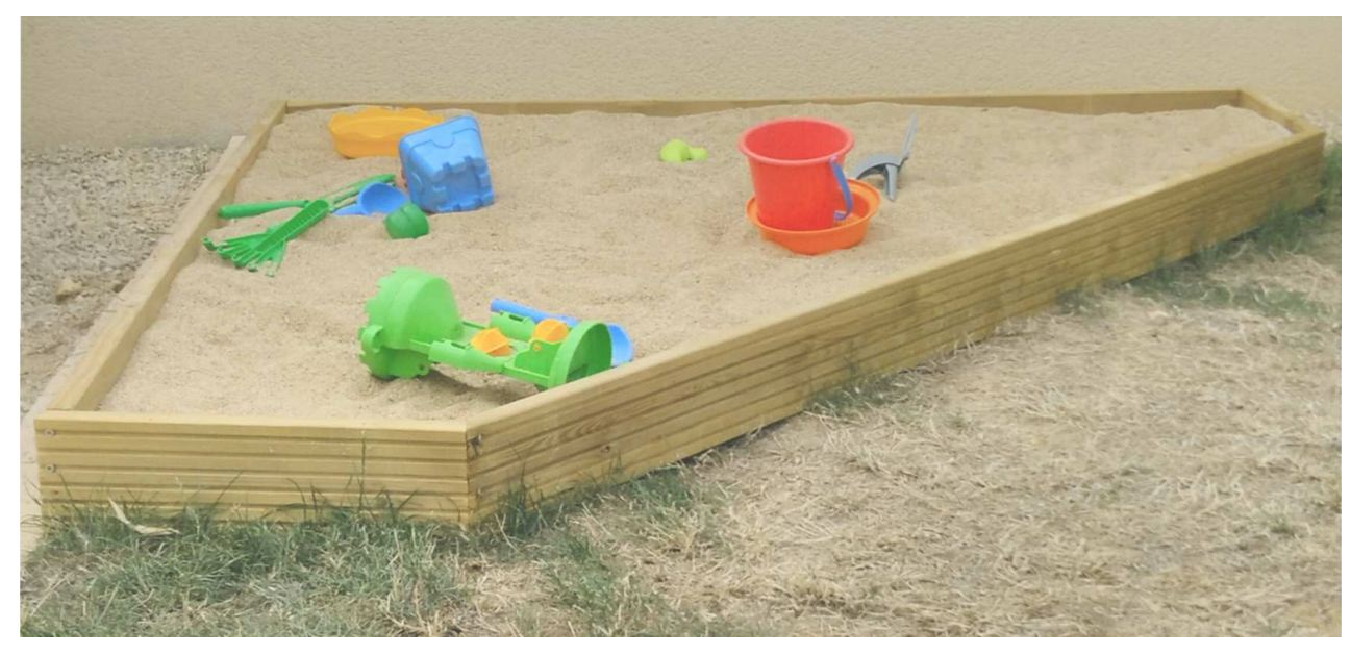
\includegraphics[width=10cm]{bac_a_sable}
\end{center}

Ce bac a la forme d'un prisme droit de hauteur $15$ cm. La base de ce prisme droit est représentée
par le polygone ABCDE ci-dessous:

\smallskip

\emph{Attention la figure n'est pas construite à la taille réelle}.

\smallskip

\begin{minipage}{0.48\linewidth}
On donne :
\begin{itemize}
\item PC = PD = 1,30 m
\item ED = BC = 40 cm
\item E, D, P sont alignés
\item B, C, P sont alignés
\end{itemize}
\end{minipage}
\hfill \begin{minipage}{0.48\linewidth}
\begin{pspicture}(5.5,5.5)
\pspolygon(2.5,0.5)(0.5,0.5)(0.5,5)(5,5)(5,3)%DEABCD
\psline[linestyle=dashed](5,3)(5,0.5)(2.5,0.5)
\psframe(0.5,0.5)(0.7,0.7)\psframe(0.5,5)(0.7,4.8)
\psframe(5,5)(4.8,4.8)\psframe(5,0.5)(4.8,0.7)
\uput[ul](0.5,5){A} \uput[ul](0.5,0.5){E} \uput[ur](5,5){B} 
\uput[r](5,3){C} \uput[d](2.5,0.5){D} \uput[dr](5,0.5){P}
\psline(1.5,0.4)(1.5,0.6) \psline(4.9,4)(5.1,4)
\psline(3.73,0.4)(3.73,0.6)\psline(3.77,0.4)(3.77,0.6)
\psline(4.9,1.73)(5.1,1.73)\psline(4.9,1.77)(5.1,1.77)
\end{pspicture}
\end{minipage}

\smallskip

\begin{enumerate}
\item Calculer CD. Arrondir au centimètre près.
\item Justifier que le quadrilatère ABPE est un carré.
\item En déduire le périmètre du polygone ABCDE. Arrondir au centimètre près.
\item On a construit le tour du bac à sable avec des planches en bois de longueur $2,40$~m et
de hauteur $15$~cm chacune. De combien de planches a-t-on eu besoin?
\item  Calculer, en m$^2$, l'aire du polygone ABCDE.
\item  A-t-on eu besoin de plus de $300$~L de sable pour remplir complètement le bac ?
\end{enumerate}
\begin{center}
\emph{Rappel : Volume d'un prisme droit $=$ aire de la base $\times$ hauteur}
\end{center}

\bigskip

